\label{chap:introduction}

\section{Background and Context}
Flooding constitutes one of the most frequent, economically catastrophic, and life-threatening natural disasters worldwide. According to the United Nations Office for Disaster Risk Reduction (UNDRR) and the Centre for Research on the Epidemiology of Disasters (CRED), floods have accounted for over 44\% of all recorded disaster events in the past two decades, impacting upwards of two billion individuals and incurring hundreds of billions of dollars in infrastructure losses. In high-density urban corridors, coastal floodplains, and riverine deltas across the Indian subcontinent and globally, flash floods and extreme monsoon deluges rapidly inundate civil infrastructure, sever primary transportation lifelines, submerge residential communities, and strand thousands of vulnerable residents within hours.

During such acute crises, rapid, accurate, and localized situational intelligence is paramount for municipal command authorities, the National Disaster Management Authority (NDMA), the National Disaster Response Force (NDRF), and international humanitarian relief agencies (such as FEMA). The fundamental bottleneck in post-disaster response has historically centered on the \textit{"Golden 72 Hours"}—the initial three-day window within which emergency search-and-rescue interventions yield the highest survivability rates. Traditional methodologies for ground damage surveying rely on physical dispatch of reconnaissance personnel, civil defense patrols, and ground vehicle expeditions. However, submerged road networks, bridge collapses, downed power transmission lines, and hazardous chemical discharges routinely render impacted zones physically inaccessible to ground survey teams, causing severe intelligence delays and blind spots.

\section{Remote Sensing and UAV Technology in Flood Management}
To overcome the physical barriers of ground reconnaissance, emergency operations centers increasingly deploy remote sensing technologies. Satellite earth observation platforms—including optical constellations (Sentinel-2, Landsat-8/9, PlanetScope) and Synthetic Aperture Radar (SAR) systems (Sentinel-1, TerraSAR-X)—provide expansive geographic coverage. Nonetheless, satellite imaging suffers from critical operational limitations in tactical emergency response:
\begin{enumerate}
    \item \textbf{Orbital Revisit Latency:} Satellite orbits impose revisit intervals varying from 24 hours to multiple days, which is incompatible with the hourly evolution of urban flash floods.
    \item \textbf{Atmospheric and Cloud Occlusion:} Optical spaceborne sensors cannot penetrate the heavy cloud decks, squall lines, and precipitation shields that inherently accompany severe meteorological events.
    \item \textbf{Coarse Spatial Resolution:} With ground sampling distances (GSD) typically ranging from 3 meters to 30 meters per pixel, spaceborne imagery lacks the resolving power necessary to detect micro-level infrastructure damage, such as submerged vehicles, single-lane flooded roadways, or individual residential structural failures.
\end{enumerate}

In contrast, small Unmanned Aerial Vehicles (UAVs or drones) have emerged as the definitive vanguard for localized post-disaster surveillance. Operating at low altitudes below cloud ceilings, UAVs capture sub-decimeter ultra-high-resolution aerial imagery (GSD $< 5\text{ cm/pixel}$) on demand. Drones can be rapidly deployed by first responders from the bed of a pickup truck, generating thousands of square meters of orthomosaic photogrammetry and video streams within minutes.

\section{Motivation and The Operational Intelligence Gap}
Despite the widespread availability of high-resolution drone imagery, disaster command centers face an acute \textit{"data-rich, information-poor"} operational dilemma. As illustrated in Figure~\ref{fig:disaster_cycle_gap}, raw aerial imagery alone does not save lives; what first responders critically require is \textbf{actionable, verified situational intelligence}. Currently, the workflow bridging raw drone video to incident response exhibits two systemic failures:

\begin{figure}[htbp]
	\centering
	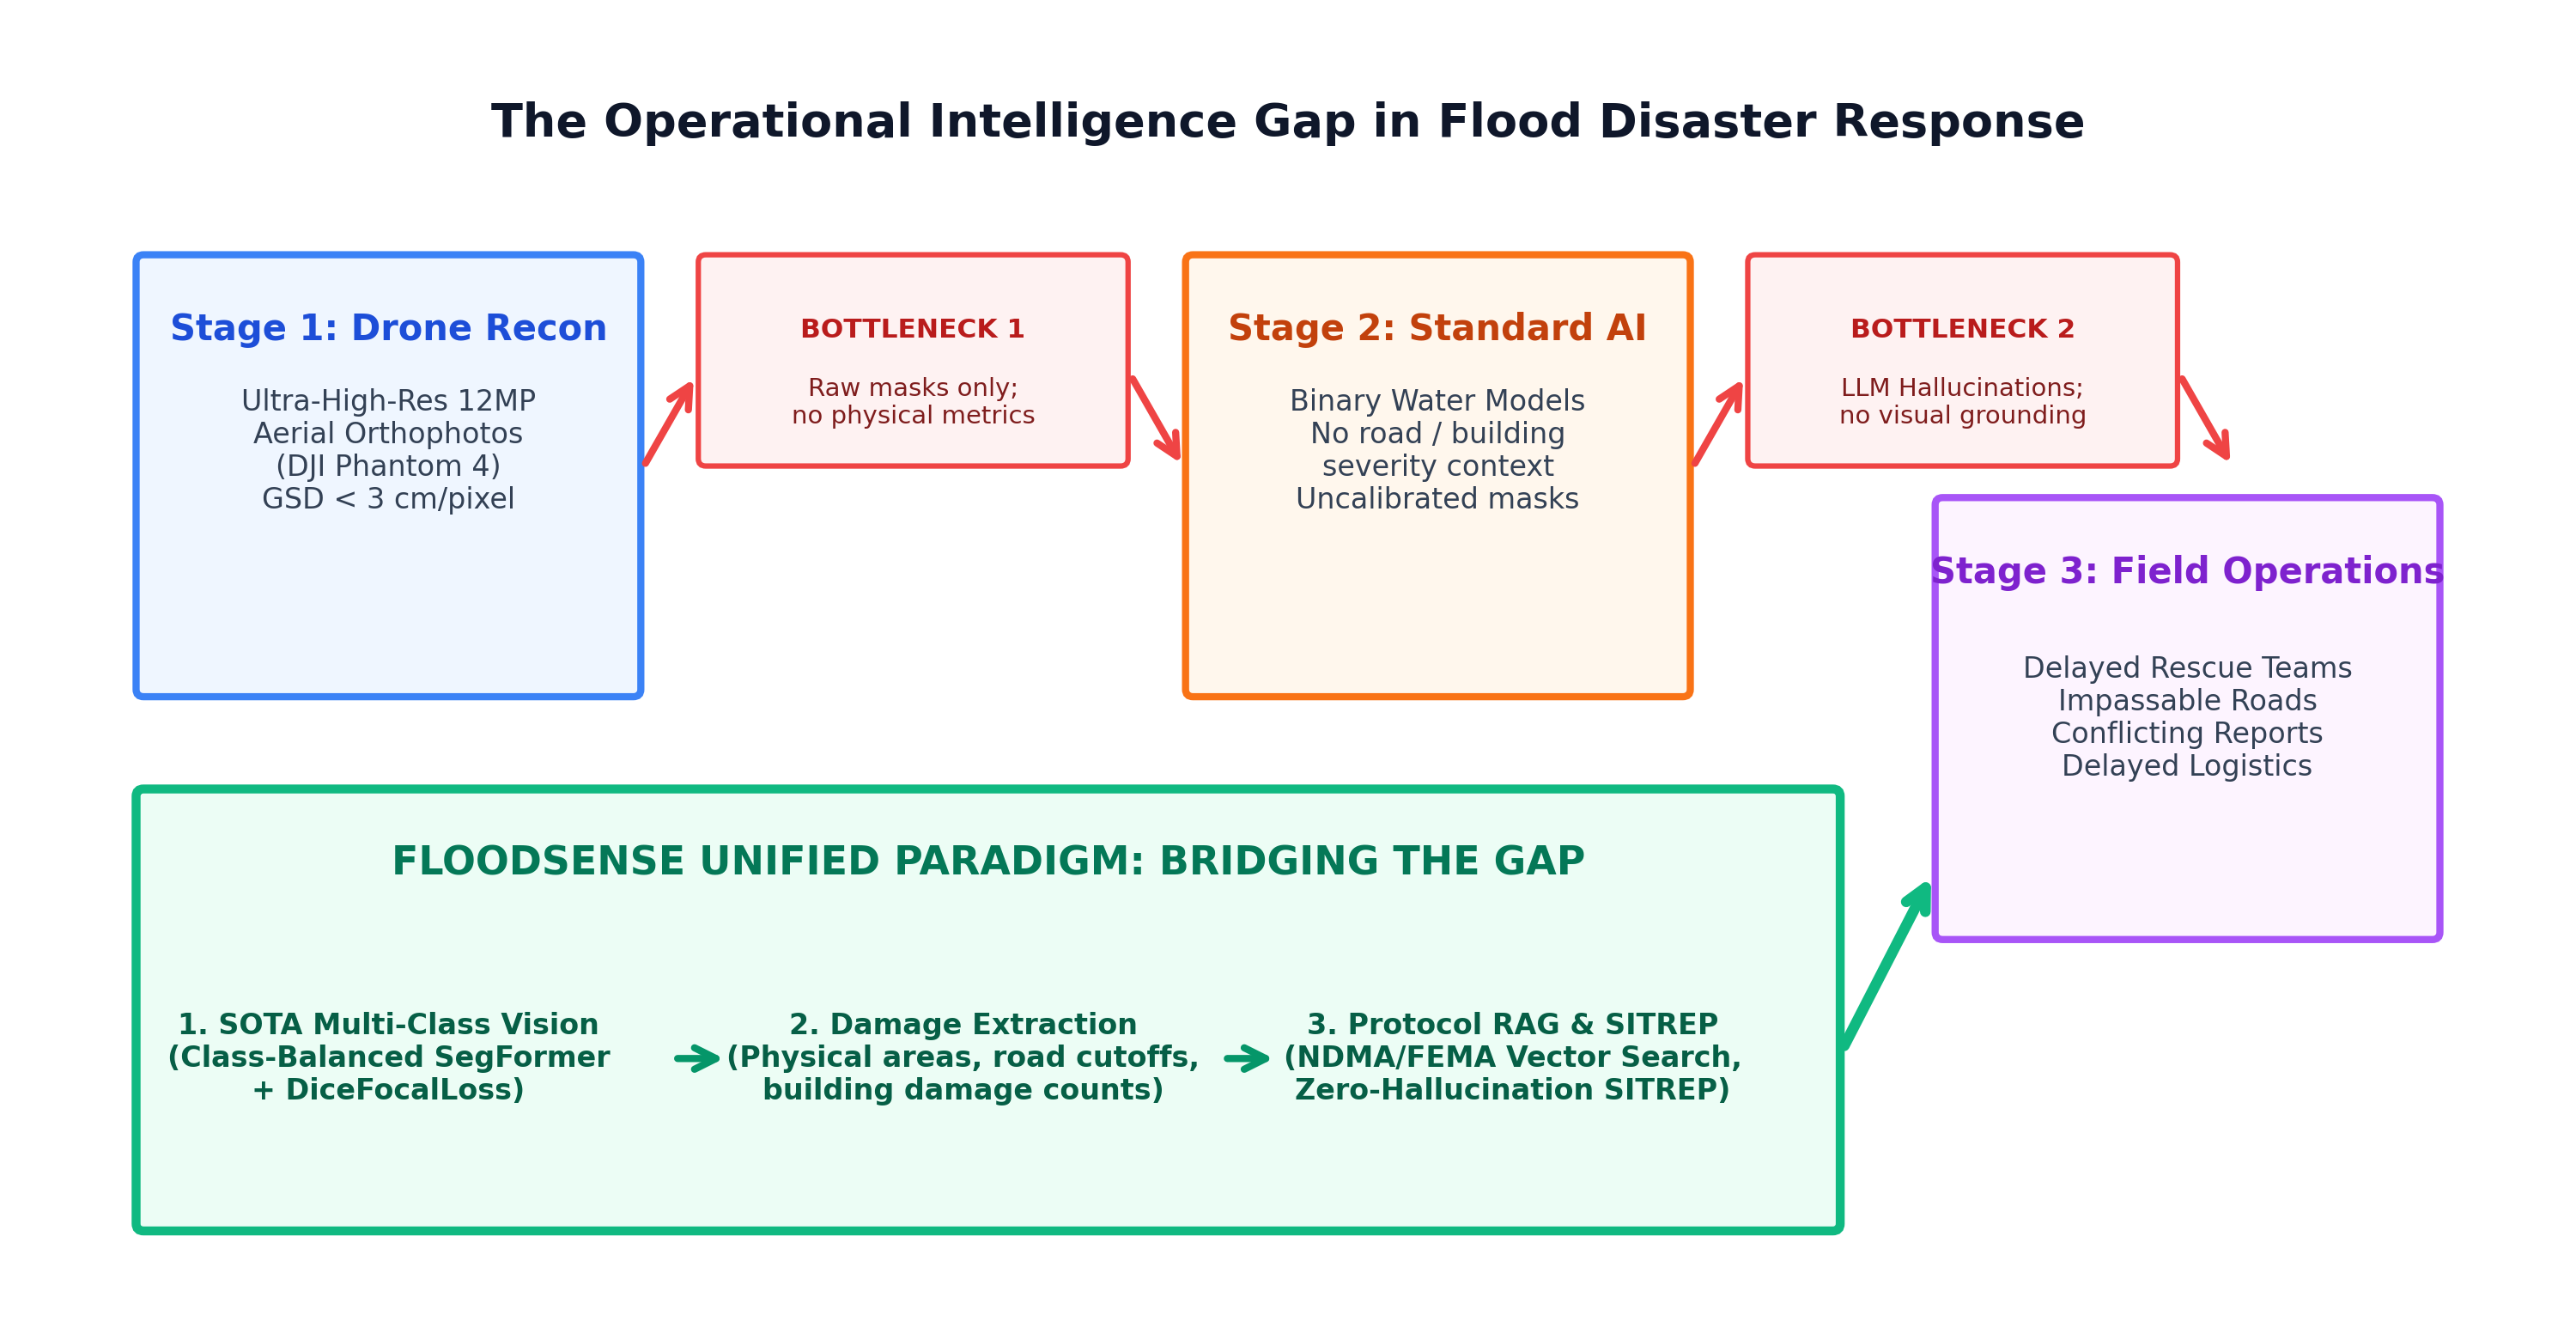
\includegraphics[width=0.92\textwidth]{images/fig1_disaster_gap.png}
	\caption{The Operational Disaster Intelligence Gap: Disconnect between aerial remote sensing, automated computer vision segmentation, statutory emergency protocols, and verifiable field reporting.}
	\label{fig:disaster_cycle_gap}
\end{figure}

\begin{itemize}
    \item \textbf{The Segmentation-to-Semantics Void:} Existing computer vision models are predominantly trained for binary water versus land delineation. In dense settlements, binary water masks fail to distinguish between flooded residential dwellings, non-flooded buildings, submerged primary transit arteries, impassable secondary streets, and stranded passenger vehicles. Furthermore, computer vision tools merely produce colorful raster overlay masks; they do not quantify physical damage, compute passable access routes, or synthesize emergency priority lists.
    \item \textbf{The Reporting-to-Protocol Void:} Conversely, newly emerging natural language disaster tools rely on Large Language Models (LLMs) to synthesize disaster summaries. However, when fed unstructured text or secondary news articles without direct visual grounding, LLMs are notoriously prone to \textit{hallucinations}—fabricating damage statistics, misidentifying neighborhood coordinates, or citing outdated emergency guidelines. In high-stakes crisis response, an ungrounded or hallucinated report can divert lifeboats to dry zones while submerged wards remain abandoned.
\end{itemize}

There is an urgent necessity for an integrated multi-modal platform that seamlessly fuses fine-grained computer vision segmentation with statutory emergency knowledge retrieval and verifiable language generation.

\section{Problem Statement}
Current post-flood disaster assessment frameworks suffer from a dichotomy of fragmented systems: visual segmentation models identify inundated regions without semantic severity interpretation or logistical reporting, while automated textual reporting engines rely on secondary web scrapers lacking verifiable visual grounding. 

The objective of this thesis is to conceptualize, benchmark, implement, and deploy \textbf{FloodSense}—an end-to-end multi-modal framework that transforms raw high-resolution UAV aerial imagery into fine-grained multi-class semantic segmentation masks, maps pixel-level spatial features into quantitative structural damage metrics, retrieves statutory disaster protocols via a dense vector-indexed Retrieval-Augmented Generation (RAG) pipeline, and generates auditable, citation-traceable Situation Reports (SITREPs) across multiple standard operational formats.

\section{Research Objectives}
To address the stated problem systematically, this research is guided by four specific technical objectives:
\begin{enumerate}
    \item \textbf{Objective 1: Multi-Paradigm Aerial Segmentation Benchmarking.} Conduct an extensive empirical benchmark across five computer vision paradigms—Classical Color-Space Thresholding, Segment Anything Model (SAM), Vision-Language Models (VLM), Zero-Shot Open-Set Detection (Grounding DINO + SAM2), and Transformer-based SegFormer—evaluating performance on the 10-class multi-class FloodNet drone benchmark.
    \item \textbf{Objective 2: Engineering a SOTA Class-Balanced High-Resolution Segmentation Pipeline.} Design and fine-tune a Transformer segmentation architecture employing class-balanced dataset sampling and a multi-objective DiceFocalLoss (combining class-weighted Focal Loss and soft Dice loss) to directly overcome acute spatial class imbalance, coupled with 2D Gaussian-feathered sliding-window inference and multi-scale dihedral Test-Time Augmentation (TTA) to preserve fine infrastructure boundaries without spatial downsampling degradation.
    \item \textbf{Objective 3: Developing a Protocol-Grounded RAG Retrieval System.} Build a dense vector retrieval pipeline utilizing sentence transformers and ChromaDB indexed across statutory disaster guidelines (NDMA, NDRF, FEMA, and historical post-disaster flood cases), attaining high retrieval precision ($Precision@1 \ge 0.90$, $Recall@3 = 1.00$, and $MRR \ge 0.95$) to govern emergency actions.
    \item \textbf{Objective 4: Multi-Format SITREP Generation and Cloud Dashboard Deployment.} Implement a deterministic, hallucination-free LLM synthesis engine that fuses extracted visual damage metrics with retrieved statutory protocol clauses into standardized disaster reports (JSON, Markdown, DOCX, PDF), and package the full framework into a responsive web dashboard suitable for field deployment.
\end{enumerate}

\section{Key Contributions of the Thesis}
The primary scientific and engineering contributions delivered in this thesis are as follows:
\begin{enumerate}
    \item \textbf{First Multi-Paradigm Benchmark on FloodNet:} We present a rigorous comparative evaluation of five distinct computer vision paradigms spanning classical, foundation, multi-modal, open-set, and fine-tuned transformer architectures on 10-class aerial flood disaster imagery.
    \item \textbf{Class-Balanced SegFormer Pipeline with DiceFocalLoss:} We propose and validate a class-balanced sampling strategy coupled with a hybrid DiceFocalLoss (fusing class-weighted Focal loss and soft multi-class Dice loss), proving its efficacy over standard cross-entropy formulations in resolving rare classes such as flooded roadways and vehicles.
    \item \textbf{Gaussian-Feathered High-Resolution Sliding Window with Dihedral TTA:} We implement an overlapping patch-inference engine that eliminates edge tiling artifacts and maintains the native ground sample distance of 12-megapixel UAV orthophotos.
    \item \textbf{Dual-Grounded Multi-Modal RAG Architecture:} We pioneer a hybrid disaster intelligence engine wherein visual damage indicators dynamically synthesize semantic queries to retrieve statutory NDMA/FEMA protocol clauses, guaranteeing zero-hallucination compliance.
    \item \textbf{Production-Grade Full-Stack System on Azure:} We demonstrate an end-to-end working system incorporating automated damage metric computation, multi-format export utilities, and a deployed interactive web dashboard backed by an enterprise Microsoft Azure Container Apps cloud architecture.
\end{enumerate}

\section{Thesis Organization}
The remainder of this thesis is structured as follows:
\begin{itemize}
    \item \textbf{Chapter 2 (Literature Survey):} Reviews state-of-the-art literature in remote sensing, deep learning segmentation, foundation vision models, Vision-Language Models, and RAG frameworks in emergency management, highlighting research gaps.
    \item \textbf{Chapter 3 (System Architecture and Problem Formulation):} Formalizes the mathematical problem statements for multi-class segmentation, spatial feature extraction, and RAG retrieval, detailing the end-to-end FloodSense architecture.
    \item \textbf{Chapter 4 (Multi-Class Aerial Image Segmentation and Benchmarking):} Explains the FloodNet UAV dataset, details the five benchmarked vision approaches, and introduces our SOTA class-balanced SegFormer pipeline with DiceFocalLoss, sliding-window inference, and TTA.
    \item \textbf{Chapter 5 (Damage Assessment, Protocol Retrieval, and Situational Intelligence):} Explains the pixel-to-metric feature conversion engine, the ChromaDB knowledge base indexing, the statutory protocol retriever, and the grounded report synthesis engine.
    \item \textbf{Chapter 6 (Experimental Results, Performance Analysis, and Discussions):} Presents exhaustive quantitative and qualitative evaluations, including ablation studies, per-class IoU/F1 comparisons, retrieval metrics, and visual comparison charts.
    \item \textbf{Chapter 7 (Interactive Dashboard and System Deployment):} Details the frontend and backend software engineering, API endpoint specifications, and live cloud deployment on Microsoft Azure.
    \item \textbf{Chapter 8 (Conclusion and Scope for Further Research):} Summarizes the primary findings, discusses operational real-world impacts, and outlines future avenues of investigation.
    \item \textbf{Appendix:} Contains complete semantic class definitions, training configuration logs, and sample disaster situation reports.
\end{itemize}
